\documentclass{article}

% if you need to pass options to natbib, use, e.g.:
%     \PassOptionsToPackage{numbers, compress}{natbib}
% before loading neurips_2021

% ready for submission
\usepackage{neurips_2021}

% to compile a preprint version, e.g., for submission to arXiv, add add the
% [preprint] option:
%     \usepackage[preprint]{neurips_2021}

% to compile a camera-ready version, add the [final] option, e.g.:
%     \usepackage[final]{neurips_2021}

% to avoid loading the natbib package, add option nonatbib:
%    \usepackage[nonatbib]{neurips_2021}

\usepackage[utf8]{inputenc} % allow utf-8 input
\usepackage[T1]{fontenc}    % use 8-bit T1 fonts
\usepackage{hyperref}       % hyperlinks
\usepackage{url}            % simple URL typesetting
\usepackage{booktabs}       % professional-quality tables
\usepackage{amsfonts}       % blackboard math symbols
\usepackage{nicefrac}       % compact symbols for 1/2, etc.
\usepackage{microtype}      % microtypography
\usepackage{xcolor}         % colors


\usepackage{amsmath}
\usepackage{graphicx}
\usepackage{tikz}
\usetikzlibrary{bayesnet}
\newcommand{\prob}[1]{\operatorname{Pr}\left[\,#1\,\right]}   
\newcommand{\expect}[1]{\operatorname{E}\left[\,#1\,\right]}   
\def\cond{\; | \;}

\title{Variational Inference for Dirichlet Process to Stratify Cancer
Patients Using DNA Methylation}

% The \author macro works with any number of authors. There are two commands
% used to separate the names and addresses of multiple authors: \And and \AND.
%
% Using \And between authors leaves it to LaTeX to determine where to break the
% lines. Using \AND forces a line break at that point. So, if LaTeX puts 3 of 4
% authors names on the first line, and the last on the second line, try using
% \AND instead of \And before the third author name.

\author{%
  David S.~Hippocampus\thanks{Use footnote for providing further information
    about author (webpage, alternative address)---\emph{not} for acknowledging
    funding agencies.} \\
  Department of Computer Science\\
  Cranberry-Lemon University\\
  Pittsburgh, PA 15213 \\
  \texttt{hippo@cs.cranberry-lemon.edu} \\
  % examples of more authors
  % \And
  % Coauthor \\
  % Affiliation \\
  % Address \\
  % \texttt{email} \\
  % \AND
  % Coauthor \\
  % Affiliation \\
  % Address \\
  % \texttt{email} \\
  % \And
  % Coauthor \\
  % Affiliation \\
  % Address \\
  % \texttt{email} \\
  % \And
  % Coauthor \\
  % Affiliation \\
  % Address \\
  % \texttt{email} \\
}

\begin{document}

\maketitle

\begin{abstract}
Variational Inference (VI) is an alternative strategy to Markov Chain Monte Carlo (MCMC) which tends to be faster and easier to scale to larger datasets (Blei et al., 2016). This is especially advantageous in applications that interact with high dimensional data. Previous work has been done on a VI method for Dirichlet Process Mixture Models (DPMMs) based on the well-known stick-breaking process (Blei and Jordan, 2006). In contrast, we propose a similar model, but based on the Chinese Restaurant Process (CRP). We hypothesize that our model will perform faster because it has fewer parameters to estimate. To test our hypothesis, we present an experiment on a large-scale stratification problem using DNA methylation to compare both implementations.
\end{abstract}

\section{Introduction}

\subsection{Variational Inference}

Variational inference is an alternative strategy to Markov Chain Monte Carlo (MCMC) sampling which tends to be faster and easier to scale to larger datasets (Blei et al., 2016). The key characteristic of variational inference is that it casts Bayesian inference as an optimization problem (Salimans et al., 2015). Variational inference attempts to approximate the posterior with another distribution $q_\theta(z|x)$ by choosing its parameters $\theta$ to optimize the evidence lower bound (ELBO) on the marginal likelihood,

%% I had to add the package amsmath, don't know if this is allowed...
\begin{align*}
\log{p(x)} &\geq \log p(x) - D_{KL}(q_\theta(z\cond x)||p(z\cond x))\\
		   &= E_{q_\theta(z\cond x)}(\log p(x,z)-\log q_\theta (z\cond x))
\end{align*}

In recent years, there have been many advances in the field of VI, which are aptly summarized in a review by Zhang et al., (2019).

\subsection{Dirichlet Process and Chinese Restaurant Process}

The Dirichlet process is a stochastic process used in Bayesian nonparametrics; a specific application being, constructing Dirichlet process mixture models (Neal, 2000). A Dirichlet process $G$ is a distribution of distributions and can be written as,

\begin{align*}
G \sim \text{DP}(G_0, \alpha)
\end{align*}

where $G_0$ is a continuous distribution such that the probability of any two samples generated from this distribution being equal is zero, whereas $G$ is a discrete distribution consisting of infinitely many number of point masses,  so the probability of two samples colliding is non-zero.  For any measurable finite k partitions $\{B_i\}_{i=1}^k$, if,
\begin{align*}
G(B_1), \cdots, G(B_k))\sim \text{Dir}(\alpha G(B_1), \cdots, \alpha G(B_k))
\end{align*}
then,
\begin{align*}
\prob{X_1, \cdots, X_k} = \int \prob{G} \prod_{i=1}^k \prob{X_i\cond G}\,dG
\end{align*}
which represents the dependencies among $\{X_i\}_{i=1}^k$ by marginalizing out $G$. \\

The Chinese restaurant process (CRP), stick-breaking process and Polya urn scheme are three common perspectives regarding the Dirichlet Process; we restrict our attention only to the Chinese restaurant process perspective in this project. The CRP can be described as follows. Assume a restaurant has infinitely many tables,  and let $\{X_i\}_{i=1}^k$ be the customers of the restaurant.  The $\{X_i\}_{i=1}^k$ are partitioned based on which table each customer is seated at.  Consider the behavior of a single customer $X_n$, given $\{X_i\}_{i=1}^{n-1}$:
\begin{align*}
X_n\cond (X_1 = x_1, X_2 = x_2, \cdots,  X_{n-1} = x_{n-1}) = \left\{
\begin{array}{rl}
x_n^* \, &\text{with probability}\ \frac{\cond\{j : x_j = n\}\cond}{n - 1 + \alpha}\\
\text{new draw from}\ G_0\, &\text{with probability}\  \frac{\alpha}{n - 1 + \alpha}
\end{array}
\right.
\end{align*}

% maybe change the notation? could be confusing
where $\cond \{j: x_j = n\}\cond$ is the number of times the value $x_n$ occurs in $\{x_1, x_2, \cdots x_n\}$.


The intuition is that customers are more likely to sit at tables with more customers, and will sit at a new table with a probability proportional to $\alpha$.\\


\subsection{Dirichlet Process Mixture Model}
The Dirichlet Process Mixture Model (DPMM) is a hierarchical model for classifying data points into an unbounded number of mixture components.  Given a sample $\{x_1, \cdots, x_N\}$, the aim of a DPMM is to compute the posterior predictive distribution, 
\begin{align*}
\prob{X = \hat{x}\cond x_1, \cdots, x_N, \alpha, G_0} = \int\prob{\hat{x}\cond x}\prob{x\cond x_1, \cdots, x_N, \alpha, G_0}\,dx,
\end{align*}
The posterior distribution $\prob{x\cond x_1, \cdots, x_N}$ does not have a closed form. Since there is an unbounded number of mixtures, sampling methods are commonly used to estimate the posterior. The most popular methods include MCMC and VI.



\subsection{DNA Methylation}

Cancers develop via the acquisition of genomic changes. These changes in turn alter the cells harbouring them, leading to changes in cell state (phenotype). One common effect of these mutations is to induce a series of modifications to the genome, which do not alter the encoded DNA but rather the ability of the DNA to be read and processed into protein. These heritable non-genetic changes are broadly referred to as epigenetic changes. According to Baylin and Jones (2011), "Epigenetic alterations are leading candidates for the development of specific markers for cancer detection, diagnosis and prognosis". One such epigenetic change is DNA methylation, which is unambiguously linked with transcriptional repression. When present in promoter regions, DNA methylation correlates negatively with gene expression; furthermore, gene promoter CpG islands acquire abnormal hypermethylation resulting in transcriptional silencing in cancer (Bock, 2012). DNA methylation can be used to stratify cancer patients into functionally similar groups. These groups can elucidate shared altered gene pathways to inform treatment strategies.


\section{Related Work}
Blei and Jordan (2006) introduced a VI algorithm for DPMMs based on the stick-breaking process. They compared the mean convergence time consumption of their VI algorithm to two MCMC sampling algorithms, i.e., Collapsed Gibbs and Blocked Gibbs. We now provide a brief description of the algorithm. Let,
%% TODO: is this correct?
\begin{align*}
\prob{G_0 = x^*\cond \lambda} = h(x^*)\exp(\lambda_1^\top x^* + \lambda_2(-a(x^*)) - a(\lambda))
\end{align*}
where $\lambda$s' are hyperparameters,  and $a(x^*)$ is a cumulant function.  Then the target function for prediction is,
\begin{align*}
\prob{x_n\cond z_n, x_1^*, x_2^*, \cdots} = \prod_{i=1}^\infty [h(x_n)\exp({x_i^*}^\top x_n - a(x_i^*))]^{\mathbf{1}[z_n = i]}
\end{align*}
This is an intractable distribution, so VI is used, along with mean-field variational approximations assuming the independence of latent variables and a derived coordinate ascent algorithm. They arrive at the following expression,
\begin{align*}
\prob{x_{N+1}\cond \ x_1, x_2, \cdots, x_{n-1}, \alpha, \lambda}\approx \sum_{t=1}^T \expect{\pi_t(\mathbf{v})}\expect{\prob{x_{N+1}\cond x_t^*}}
\end{align*}
% TODO: q isn't even in the equation?
where $q$ is an approximation to the predictive distribution depending on $x_1, x_2, \cdots, \alpha, \lambda$,  and each component $v_i$ in $\mathbf{v}$ follows the beta distribution with parameters $(1, \alpha)$.

\section{Methods}
\subsection{Model}
% TODO: is that the right way to cite?
% TODO: maybe cite pyro?
This paper builds upon Blei and Jordan's work (2006). We propose a VI algorithm for DPMMs based on a CRP, to stratify cancer patients using DNA methylation. Our method differs in that we base our model on a CRP as opposed to a stick-breaking process. We will use the probabilistic programming language Pyro to implement both models (see Figure 1 for graphical models).

\begin{figure}[!htp]
	\centering
	\begin{minipage}{0.45\textwidth}
		\centering
		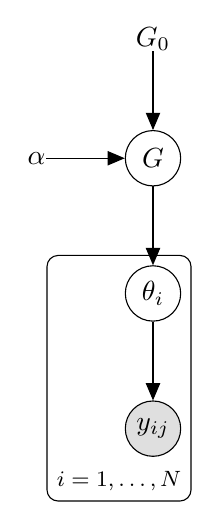
\begin{tikzpicture}
		  \node[obs] (y) {$y_{ij}$} ; % 
		  \node[latent, above=of y](theta){$\theta_i$} ; %
		  \node[latent, above=of theta] (G) {$G$} ; %
		  \node[const, above=of G] (G0) {$G_0$} ; %
		  \node[const, left=of G] (alpha) {$\alpha$} ; %
		
		  
		
		  \edge{G0}{G}
		  \edge{alpha}{G}
		  \edge{G}{theta}
		  \edge{theta}{y}
		  
		  
		  \plate {patients} { %
		    (y)(theta) %
		  } {$i=1,\ldots,N$} ; %
		\end{tikzpicture}
		\caption{Graphical model for DPMM based on CRP}
	\end{minipage}\hfill
	\begin{minipage}{0.45\textwidth}
		\centering
		\vspace{1.35cm}
		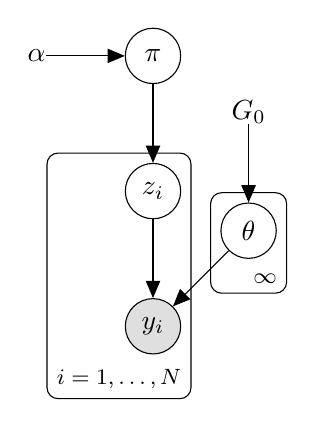
\begin{tikzpicture}
		  \node[obs] (y) {$y_{i}$} ; % 
		  \node[latent, above=of y] (z) {$z_i$} ; %
		  \node[latent, above=of z] (pi) {$\pi$} ; %
		  \node[const, left=of pi] (alpha) {$\alpha$} ; %
		  \node[latent, above right=of y] (theta) {$\theta$} ; %
		  \node[const, above=of theta] (G0) {$G_0$} ; %
		  
		
		  \edge{G0}{theta}
		  \edge{theta}{y}
		  \edge{z}{y}
		  \edge{pi}{z}
		  \edge{alpha}{pi}
		  
		  
		  \plate {patients} { %
		    (y)(z) %
		  } {$i=1,\ldots,N$} ; %
		  
		  \plate{clust_params}{
		   (theta)}{$\infty$}
		\end{tikzpicture}
		\caption{Graphical model for DPMM based on the stick-breaking process}
	\end{minipage}
\end{figure}

\subsection{Data Preprocessing}
DNA methylation data will be obtained from the International Cancer Genome Consortium (ICGC) and processed in R. Preprocessing steps will include:

\begin{itemize}
\item Filtering / Cleaning
\item Probe to gene mapping using FDb.InfiniumMethylation.hg19 (Triche, 2014)
\item Normalization
\item Dimensionality reduction
\end{itemize}



\section{Expected Results}
\subsection{Clustering}
We intend to use clustermaps where color bars on the left hand side indicates cancer type and purple squares represent the clusters. The more data points in the cluster, the larger the squares. The intensity of a square describes the proportion of iterations the data point of interest appeared in that cluster. We expect that our clustermaps will resemble Figure 3, as patients should cluster by cancer type.

\begin{figure}[!htp]
	\centering
	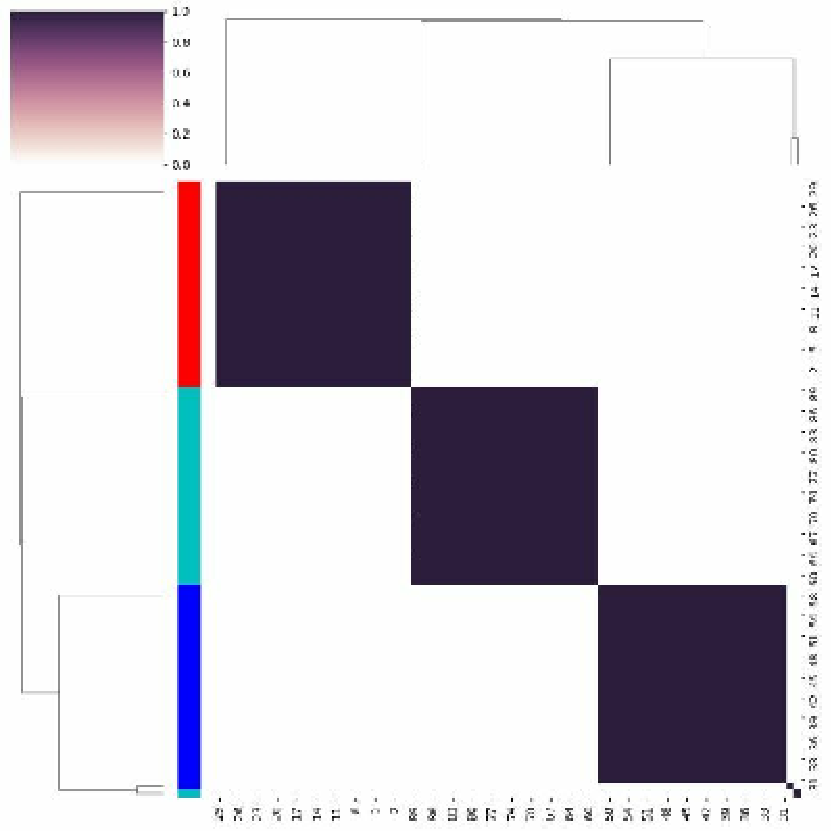
\includegraphics[scale=0.3]{figures/example_clustermap.pdf}
	\caption{Example of a clustermap. Color labels indicate cancer types: \color{red}{Type I}, \color{blue}{Type II}, \color{cyan}{Type III}}
\end{figure}


\subsection{Mean Convergence Time}
We expect to observe that our model, based on a CRP will have a shorter mean convergence time compared to Blei and Jordan's model. Plots depicting the relationship between dimension, time, and algorithm type will be used to visualize and evaluate our hypothesis. We expect that our plot will look similar to Figure 4, and will show that our model performs faster than Blei and Jordan's. 

\begin{figure}[!htp]
	\centering
	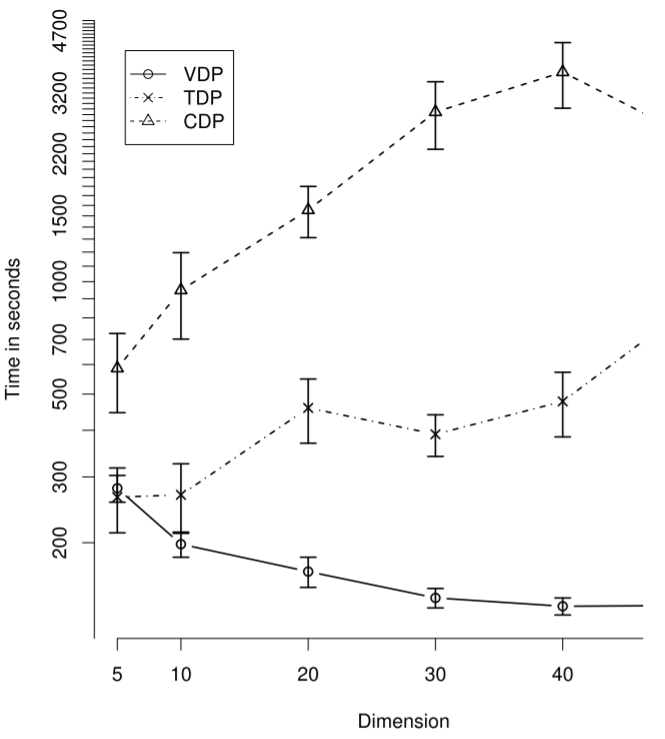
\includegraphics[scale=0.3]{figures/speed.png}
	\caption{Mean convergence time and standard error across ten data sets per dimension for variational inference, TDP Gibbs sampling, and the collapsed Gibbs sampler (Blei and Jordan, 2006)}
\end{figure}



\section*{References}

\medskip
{
\small

[1] Baylin, Stephen B., and Peter A. Jones.  A Decade of Exploring the Cancer Epigenome -- Biological and Translational Implications.  {\it Nature Reviews Cancer}, vol 11, no. 10, 23 Sept. 2011, pp. 726-734, 10.1038/nrc3130.

[2] Blei, David M, et al. Variational Inference: A Review for Statisticians. {\it Journal of the American Statistical Association}, vol. 112, no. 518, 27 Feb. 2017, pp. 859-877, arxiv.org/abs/1601.00670, 10.1080/01621459.2017.1285773.

[3] Blei, David M., and Michael I. Jordan. Variational Inference for Dirichlet Process Mixtures. {\it Bayesian Analysis}, vol.1, no.1, Mar.2006, pp. 121-143, 10.1214/06-ba104.

[4] Bock, Christoph, et al. Quantitative Comparison of Genome-Wide DNA Methylation Mapping Technologies. {\it Nature Biotechnology}, vol. 28, no. 10, 19 Sept. 2010, pp. 1106-1114, 10.1038/nbt.1681.

[5] Salimans, Tim, et al.  Markov Chain Monte Carlo and Variational Inference: Bridging the Gap. ArXiv: 1410.6460, 19 May 2015, arxiv.org/abs/1410.6460.

[6] Zhang, Cheng, et al. Advances in Variational Inference. {\it IEEE Transactions on Pattern Analysis and Machine Intelligence}, vol. 41, no. 8, 1 Aug. 2019, pp. 2008-2026, 10.1109/tpami.2018.2889774.

[7] Triche, Jr. T (2014). FDb.InfiniumMethylation.hg19: Annotation package for Illumina Infinium DNA methylation probes. R package version 2.2.0.
}

\end{document}